\section{Magnitudes Extensivas}

Se llama extensivas a las variables que son cuantificables y existen o son contenidas dentro del sistemas. Estas dependen de la cantidad de materia de modo que varían de forma directamente proporcional al tamaño de sistema.

\begin{itemize}
    \item Al estar contenidas en una región del espacio, se les puede asociar una densidad volumétrica.
    \item Toda magnitud extensiva es aditiva.
    \item Al trasladar un sistema, se transportan con él las magnitudes extensivas que contiene. esto permite definir corrientes.
\end{itemize}

\subsection{Magnitudes Intensivas}

En contraposición de las magnitudes extensivas están las intensivas que no dependen de la cantidad de materia, son intrínsecas.

\section{Sistemas Termodinámicos}

Se llama sistema a la región del espacio que se observa o estudia. Se distinguen tres tipos de sistemas:

\begin{itemize}
    \item \textbf{Aislado:} no intercambia magnitudes extensivas con el medio. Posee paredes adiabáticas (impiden el flujo de calor) , impermeables e inmóviles.
    \item \textbf{Cerrado:} permite en intercambio de energía con el medio. Poseen paredes diatérmicas (admiten el flujo de calor) e impermeables.
    \item \textbf{Abierto:} Permite el intercambio de energía con el medio
\end{itemize}

\subsection{Baño Térmico}

Se llama baño térmico o fuente a un sistema de tamaño mucho mayor que el del sistema de interés y que se encarga de suministrarle calor, manteniéndose a temperatura constante (su variación es despreciable).\\
Se dice que tiene capacidad calórífica o térmica ``infinita''.

\subsection{Microestados y Macroestados}

\textbf{Microestados:} distintas configuraciones que puede adoptar un sistema. El número de microestados posibles de un sistema se representa por la función $\Omega(E, N, V)$.\\

\textbf{Macroestados:} conjunto de microestados.

\subsection{Energía Interna}

La energía interna de un sistema corresponde a la suma de energía mecánica de las partículas que lo componen. Generalmente no es constante y posee una variación menor a lo medible con un instrumento típico. Se suele usar el promedio como energía interna.

\subsection{Entropía}

%Definición cualitativa de la entropía 

\textbf{Entropía de Boltzmann}

\[S(E,N,V) = k_B\ln{(\Omega(E,N,V))}\]

\subsection{Variables de Estado}

Se llama variable o función de estado a cualquier cantidad física que tiene un valor definido para cada estado de equilibrio del sistema y se puede expresar como una función de las demás variables de estado. En equilibrio térmico estas variables no dependen den tiempo, dependen sólo del estado termodinámico actual y no de como se llego hasta él.
\medbreak
Si un sistema está descrito por parámetros $x=(x_1, x_2, ...)$, para $f(x)$ una función de estado, se verifica que en un cambio de parámetros de $x_i$ a $x_f$, el cambio en $f(x)$ es

\[\Delta f = \int^{x_f}_{x_i}df = f(x_f)-f(x_i)\]

donde $df$ es un diferencial exacto, por lo que $\Delta f$ depende sólo de $x_f$ y $x_i$.

\section{Segunda Ley de la Termodinámica}
\label{2ley}
La entropía de un sistema aislado no decrece con el tiempo y es constante si y sólo si todos los procesos son reversibles.\\

También puede establecerse la segunda ley de las siguientes formas (siempre en un sistema aislado):
\begin{itemize}
    \item \textit{La entropía se puede crear, pero no se puede aniquilar}
    \item \textit{En un sistema aislado el estado de equilibrio es el de entropía máxima}
\end{itemize}

\textbf{Enunciado Microscópico:} en un sistema aislado, si se libera una restricción para las variables de estado, estas evolucionarán al valor que maximice la entropía de Boltzmann.\\

\textbf{Relación con máquinas térmicas:} \textit{NO} existe máquina térmica (motor) con rendimiento mayor al de Carnot. \label{2ley-motor}\\

\textbf{Formulación de Clausius:} no existe proceso cuyo único efecto sea transferir calor de un cuerpo frío a otro caliente.\\

\textbf{Enunciado de Kelvin:} no existe proceso cuyo único efecto sea extraer energía de un baño térmico (calor) y transformarlo en trabajo.

\section{Calor}

Flujo de energía entre cuerpos a distinta temperatura.

\subsection{Capacidad Calorífica o térmica}

Calor necesario para aumentar la temperatura de un objeto en una cierta cantidad. Es una magnitud extensiva.

\[C = \frac{dQ}{dT}\]

En baño térmico $C$ es lo suficientemente grande como para que no experimente cambios apreciables en su temperatura.

\subsection{Calor específico}

Calor necesario para aumentar la temperatura de una unidad de masa. Es una magnitud intensiva.

\[c = \frac{C}{m} = \frac{1}{m}\frac{dQ}{dT}\]

\section{Primera ley de la Termodinámica}
\label{1ley}
La energía interna de un sistema aislado es constante.

\subsection{En Términos de Calor y Trabajo}

El cambio de energía interna de un sistema $\Delta E$ es

\[\Delta E = Q+W\]

\begin{itemize}
    \item Si $Q>0$, se suministra calor al sistema y si $Q<0$ se extrae de este.
    \item Si $W>0$ se ejerce trabajo sobre el sistema y si $W<0$ el sistema ejerce trabajo sobre el medio.
    \item Para $\Delta V$ el cambio de volumen, se verifica que $w\Delta V < 0$.
\end{itemize}

\textbf{Forma Diferencial:}

\[dE = \di W+ \di Q\]

\section{Procesos Termodinámicos}

Cuando un sistema cambia de un estado de equilibrio termodinámico a otro, decimos que ocurrió un proceso.
\[(ETD)_1 \xrightarrow[]{\text{proceso}} (ETD)_2 \]

\textbf{Proceso reversible}: se definen como aquellos en donde el cambio de entropía luego de ocurrido el proceso es cero, \textit{\enquote{Se conserva la entropía}}. Un sistema que experimenta un proceso reversible es capaz de volver por sí mismo al estado original.
\\

\textbf{Proceso irreversible}: son aquellos procesos en los cuales al pasar de un (ETD) a otro existe cambio de entropía (aumenta). También se puede establecer que durante el proceso el sistema está fuera del equilibrio. Si $\Delta E_B > 0$ el proceso es irreversible. $\Sigma_r+\Sigma_d$ corresponde a la energía disipada que se va al baño y es irrecuperable.
\\

\textbf{Proceso cuasi-estático (PCE)}: si un sistema de interés va cambiando durante un proceso, de manera que a todo instante sus variables de estado están definidas (un único valor para el sistema), y se relacionan entre sí estas variables por las ecuaciones de estado, entonces decimos que el proceso es cuasi-estático. \\


En un PCE el trabajo puede ser máximo o mínimo dependiendo si es el que se extrae o el que se hace sobre el sistema.

\begin{itemize}
    \item[-] Cuando es el que se hace sobre el sistema es el trabajo mínimo paraa lograr la transformación
    \item[-] Cuando es el extraído es el máximo trabajo extraíble en la transformación. 
    
    \begin{equation}
    \begin{split}
        \text{proceso reversible} &\implies PCE\\
        &\centernot\Longleftarrow
    \end{split}
    \nonumber
\end{equation}
\end{itemize}

\textbf{Equilibrio para un sistema}: cuando sus variables de estado (\textit{S, E, N, V, p, T, ...}) se relacionan por las ecuaciones de estado.\\

\textit{Dos fronteras están en equilibrio entre sí, si $T_1 = T_2$ cuando la pared es diatérmica, o si $p_1 = p_2$ cuando la pared es móvil.}

\subsection{Ciclos}
\label{ciclos}
Un ciclo es una serie proceso en el que se regresa al estado inicial (esto no implica que sean reversibles).\\

\textbf{Ciclo de Carnot:} Ciclo reversible que reversible que involucra 2 baños térmicos en el que se repiten los siguientes procesos:

\begin{itemize}
    \item En contacto con el baño 2 se aumenta la entropía de $S_1$ a $S_2$
    \item En un proceso adiabático ($\Delta S=0$) se baja la temperatura de $T_2$ a $T_1$
    \item En contacto con el baño 1 se disminuya la entropía de $S_2$ a $S_1$
    \item En un proceso adiabático se aumenta la temperatura de $T_1$ a $T_2$
\end{itemize}

El ciclo de Carnot recorrido en este sentido constituye un motor que minimiza la energía disipada y maximiza el trabajo extraído. Recorrido en el sentido inverso forma un refrigerador.

\begin{itemize}
    \item \textbf{Temperaturas absolutas:} el ciclo se Carnot permite definir temperaturas independientes del sistema. Se fija una temperatura $T_2$, y se define $T_1$ como
\[T_1 = T_2(1-\eta_c)\]
\end{itemize}

\subsection{Motores}

En un motor se realiza un ciclo con dos baños térmico, uno caliente y otro frío, que permite extraer trabajo ($W<0$).\\

\begin{minipage}{0.5\textwidth}%
\begin{figure}[H]
    \centering
    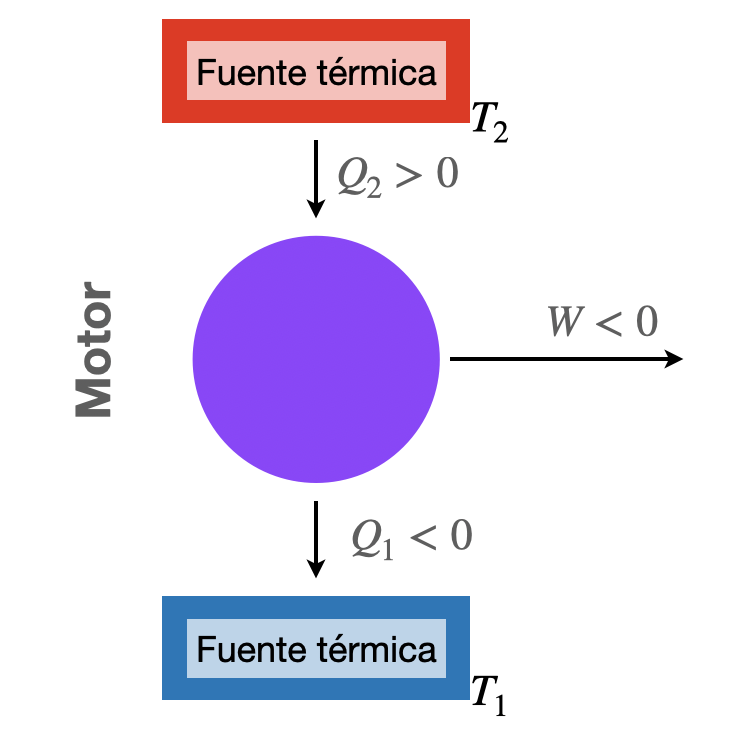
\includegraphics[width=0.87\textwidth]{img/motor_carnot.png}
    \caption{Motor}
    \label{fig:motor}
\end{figure}
\end{minipage}%
\begin{minipage}{0.5\textwidth}%
\begin{figure}[H]
    \centering
    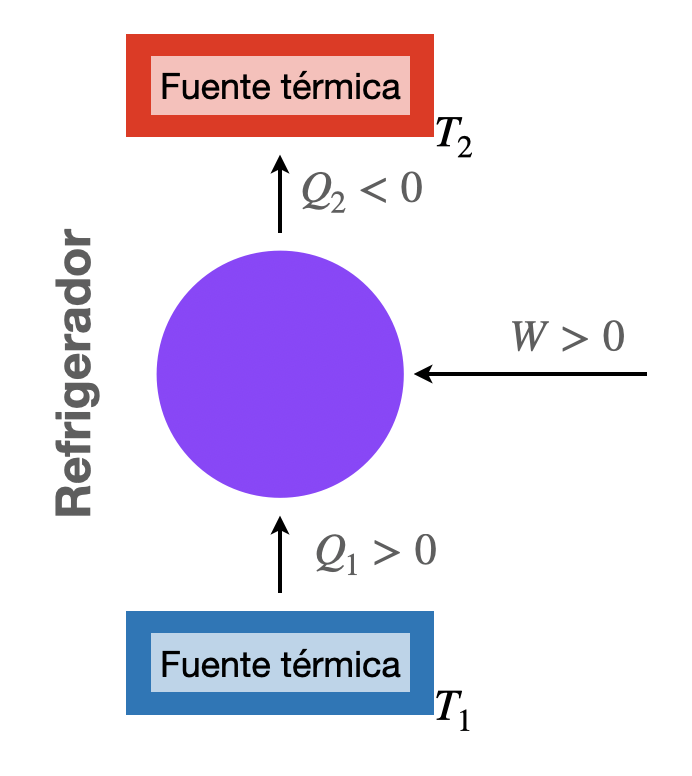
\includegraphics[width=0.79\textwidth]{img/refrigerador.png}
    \caption{Refrigerador o bomba térmica}
    \label{fig:refrigerador}
\end{figure}
\end{minipage}%
\hfill\\

Un refrigerador o bomba térmica, es un motor inverso del al cual se le inserta trabajo para aumentar la temperatura de un baño térmico \enquote{más frío}. ($W >0$)\\

\textbf{Análisis lógico de un motor}:\label{plbr-motor}
en la ecuación $\eta = \frac{-W}{Q_2}$ se tiene que $W$ es lo que queremos obtener y $Q_2$ lo que invertimos.\\

\textbf{Refrigeradores - $Q_2$ y $W$}:
\label{refri-q2-w}
se tiene que en un refrigerador o bomba térmica (realizan lo mismo) se tiene la relación
\[\abs{Q_2} = (1 + \eta^R)W\]
Donde \enquote{la mejor} estufa cumple que $\abs{Q_2} = W$

\section{Ley cero de termodinámica}
% Falta información ?

Dos sistemas, cada uno por separado en equilibrio con un tercero, están en equilibrio entre sí.

\textit{Si un cuerpo ’A’ está en equilibrio con uno ’B’, y ’B’ está en equilibrio con ’C’, entonces ’A’ está en equilibrio con ’C’.}

\section{Formalismo termodinámico o potenciales termodinámicos}

\textbf{Entropía}: $S(E, V)$ es un potencial termodinámico.
\[\implies \frac{1}{T(E,V)} = \devtermo{V}{S}{E} \quad 
\land \quad \frac{p(E,V)}{T} = \devtermo{E}{S}{V}\]

\textbf{Energía}: $E(S,V)$ es un potencial termodinámico.
\[\implies T(S,V) = \devtermo{V}{E}{S} \quad \land \quad p(S,V) = -\devtermo{S}{E}{V}\]

Teniendo en cuenta que si tenemos $S = S(T, V)$, entonces $\frac{p}{T} \neq \devtermo{T}{S}{V}$\\

\textbf{Variables naturales}: son las variables que si se usan para determinar cierta propiedad del sistema (S, E, F, etc) permiten obtener el resto de variables del termodinámicas del sistema.\\

Además causan que en equilibrio termodinámico, las variables definidas sean mínimas, a excepción de la entropía, que causa que sea máxima.\\

Todas las funciones (Entropía, Energía, Energía libre de Helmholtz, etc) estarán definidas en función a sus variables naturales en esta sección.\\

Si es que algunas de las funciones o su diferencial se puede expresar en relación a otras dos variables provenientes de su definición, entonces se tendrá que también serán variables naturales. (e.g. $dF = dE - TdS - SdT$, sea $dE = \gamma dA + TdS$ entonces $dF = \gamma dA - SdT$ y $F = F(A,T)$).\\

\textbf{Energía libre de Hemholtz (o potencial, o función)}: $F = F(T,V)=E-TS$ es un potencial termodinámico ($dE = -pdV - sdT$)

\[\implies \devtermo{T}{F}{V} = -p \quad \land \quad \devtermo{V}{F}{T} = -S\]

\textbf{Entalpía}: $H =H(S,p)=E+pV$ es un potencial termodinámico ($dH = TdS + Vdp$)

\[\implies \devtermo{p}{H}{S} = T \quad \land \quad \devtermo{S}{H}{p} = V\]



\textbf{Relaciones de Maxwell}: \label{relaciones-maxwell} hacen uso de que los potenciales termodinámicos son de clase $\mathcal{C}^2$, por lo que sus segundas derivadas parciales con respecto a dos variables son iguales sin importar el orden de derivación. 

\begin{itemize}
    \item Para la energía:
    \[\devtermo{S}{T}{V} = -\devtermo{V}{p}{S}\]
    \item Para la energía libre de Helmholtz:
    \[\devtermo{V}{p}{T} = \devtermo{T}{S}{V}\]
    \item Para la entalpía:
    \[ \devtermo{S}{T}{p} = \devtermo{p}{V}{S} \]
\end{itemize}

\newpage